\section{AFL++ Status Screen Results for the Different modes}
\setcounter{figure}{0}

\begin{figure}[h!]
\centering
\begin{subfigure}{0.48\textwidth}
    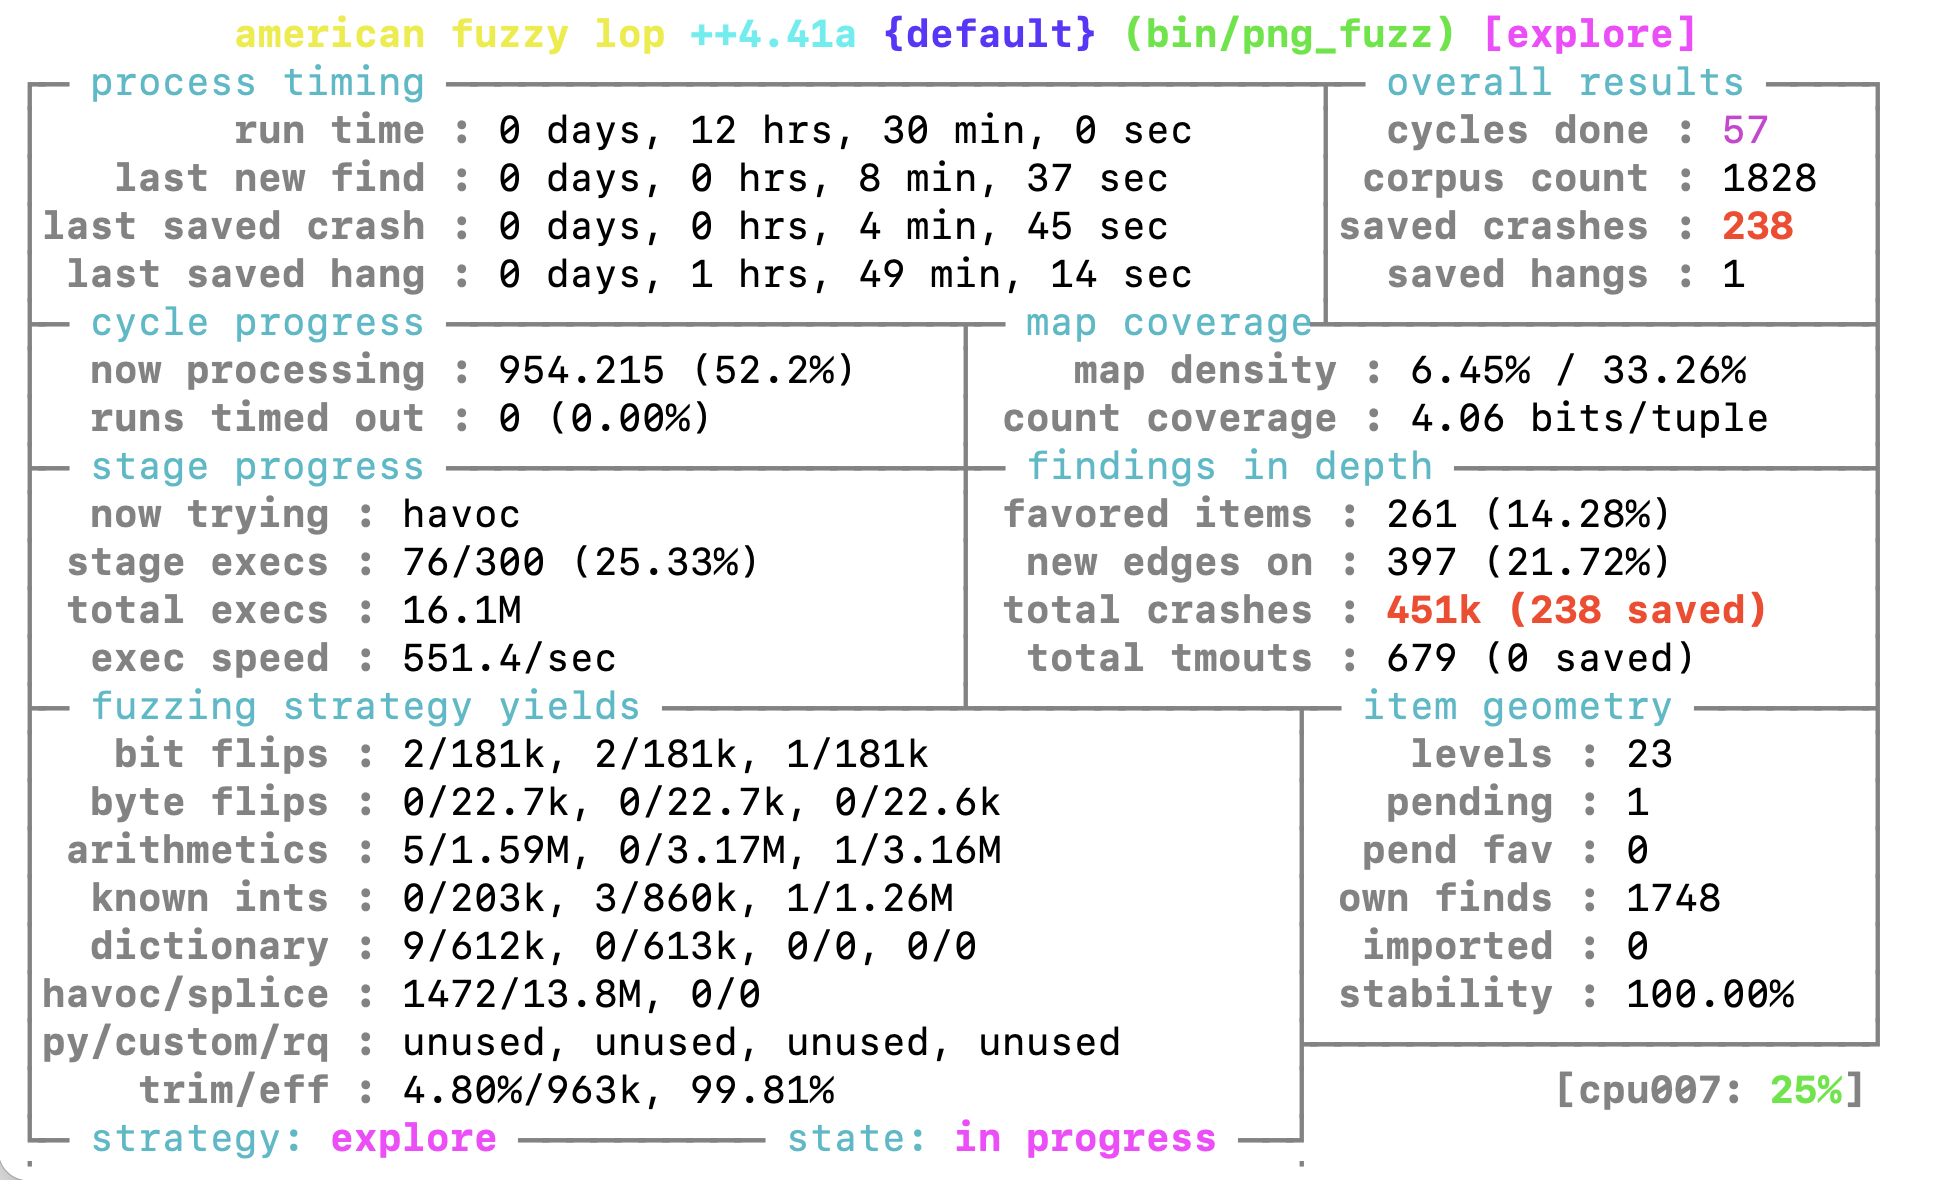
\includegraphics[width=1\linewidth]{figures/AFL_status_fork.png}
    \caption{}
    \label{fig:status_fork}
\end{subfigure}
\begin{subfigure}{0.48\textwidth}
    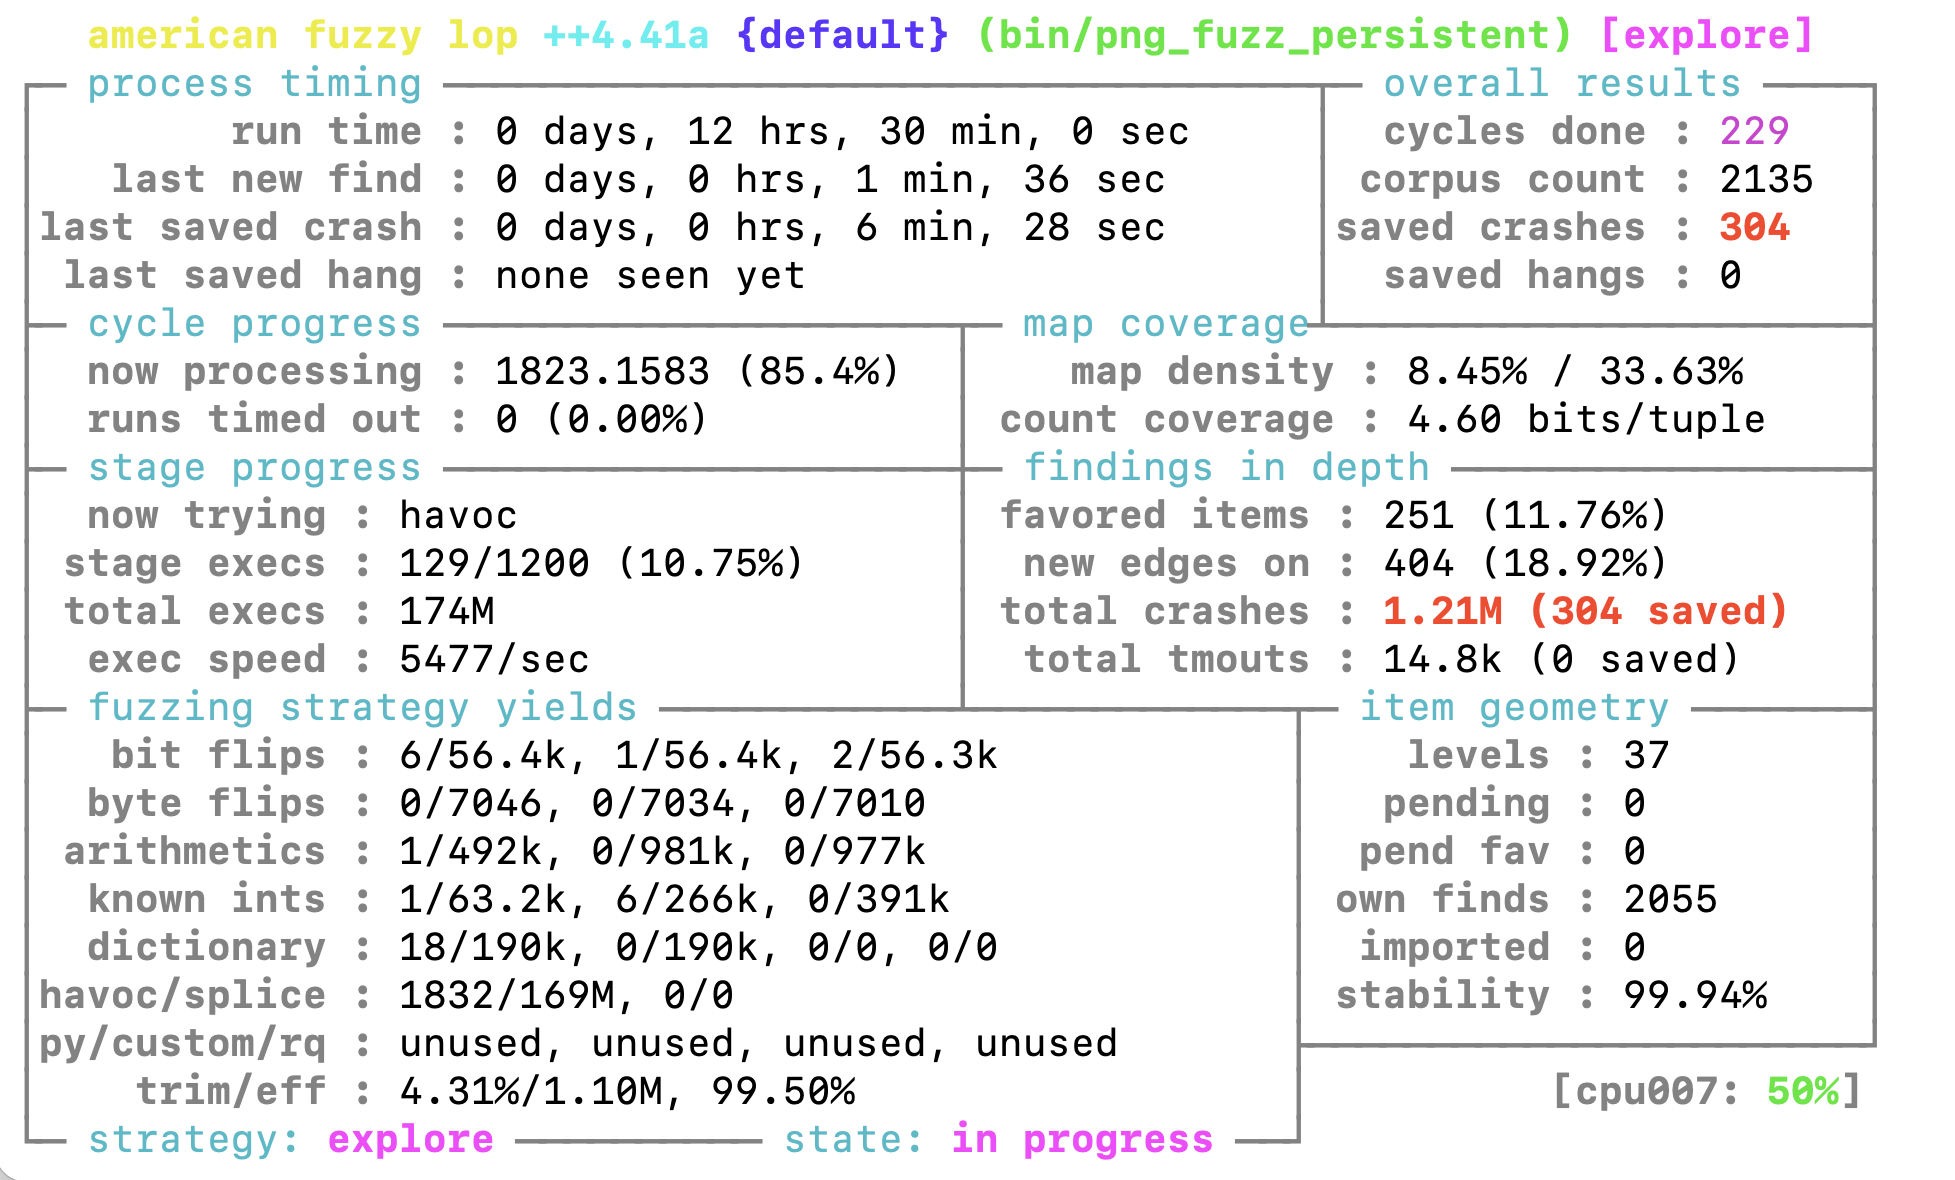
\includegraphics[width=1\linewidth]{figures/AFL_status_persistent.png}
    \caption{}
    \label{fig:status_persistent}
\end{subfigure}
\begin{subfigure}{0.48\textwidth}
    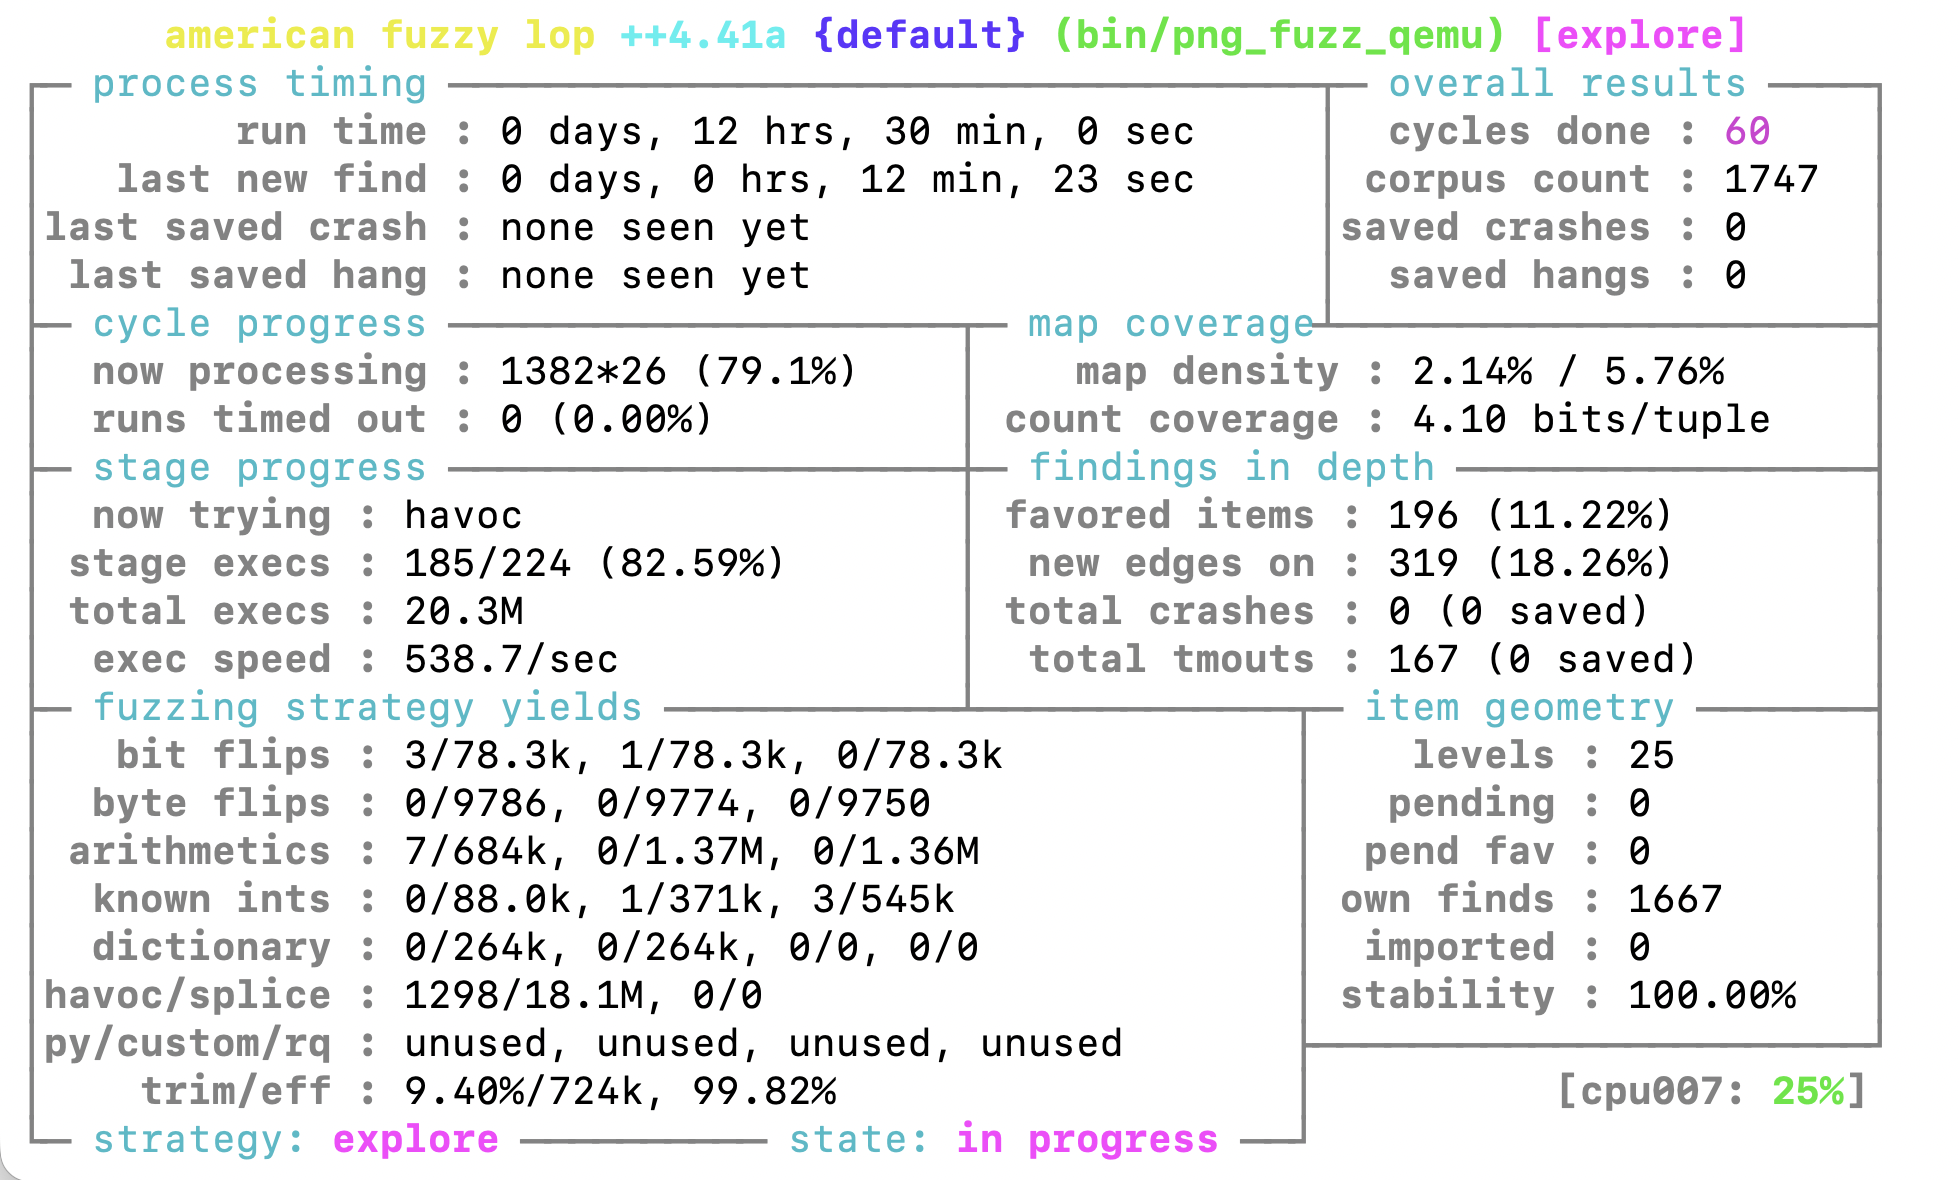
\includegraphics[width=1\linewidth]{figures/AFL_status_qemu.png}
    \caption{}
    \label{fig:status_qemu}
\end{subfigure}
    \caption{AFL++ status screen for the campaign of (a) and (b) the instrumented libpng library, with respectively the persistent was disabled and enabled, (c) the un-instrumented binary (qemu mode). All the campaign durations were 12 h 30 min. All three campaigns have been run simultaneously the same machine on three different CPU, so they were all subject to the same system conditions and are therefore directly comparable in terms of performance.}
    
\end{figure}
%======================================================
\newpage
\section{Fuzzing Campaign Results}
\subsection{For ASan and fork mode}
\setcounter{figure}{0}
\begin{figure}[h!]
\centering
\begin{subfigure}{0.75\textwidth}
    
\includegraphics[width=\textwidth]{figures/plot_output/edges}
    \caption{}
    \label{fig:fork_edges}
\end{subfigure}
\begin{subfigure}{0.75\textwidth}
    
\includegraphics[width=\textwidth]{figures/plot_output/exec_speed}
    \caption{}
    \label{fig:fork_exec_speed}
\end{subfigure}
\begin{subfigure}{0.75\textwidth}
    
\includegraphics[width=\textwidth]{figures/plot_output/high_freq}
    \caption{}
    \label{fig:fork_high_freq}
\end{subfigure}
\begin{subfigure}{0.75\textwidth}
    
\includegraphics[width=\textwidth]{figures/plot_output/low_freq}
    \caption{}
    \label{fig:fork_low_freq}
\end{subfigure}
\caption{Afl-plot data analysis of the campaign for the instrumented binary, with fork mode, for different metrics : (a) the number of edges, (b) the execution per second, (c) and (d) time evolution of different elements. The two gaps in the execution per second have been produced by the accidental sleep mode of the computer.}
\label{fig:plot_data_fork}
\end{figure}
%======================================================
\newpage
\subsection{ASan with Persistent Mode}

\begin{figure}[h!]
\centering
\begin{subfigure}{0.75\textwidth}
    
\includegraphics[width=\textwidth]{figures/plot_output_persistent/edges}
    \caption{}
    \label{fig:persistent_edges}
\end{subfigure}
\begin{subfigure}{0.75\textwidth}
    
\includegraphics[width=\textwidth]{figures/plot_output_persistent/exec_speed}
    \caption{}
    \label{fig:persistent_exec_speed}
\end{subfigure}
\begin{subfigure}{0.75\textwidth}
    
\includegraphics[width=\textwidth]{figures/plot_output_persistent/high_freq}
    \caption{}
    \label{fig:persistent_high_freq}
\end{subfigure}
\begin{subfigure}{0.75\textwidth}
    
\includegraphics[width=\textwidth]{figures/plot_output_persistent/low_freq}
    \caption{}
    \label{fig:persistent_low_freq}
\end{subfigure}
        
\caption{Afl-plot data analysis of the campaign for the instrumented binary, with persistent mode, for different metrics : (a) the number of edges, (b) the execution per second, (c) and (d) time evolution of different elements. The two gaps in the execution per second have been produced by the accidental sleep mode of the computer.}
\label{fig:plot_data_persistent}
\end{figure}

%======================================================
\newpage
\subsection{Qemu Mode}
\begin{figure}[h!]
\centering
\begin{subfigure}{0.75\textwidth}
    
\includegraphics[width=\textwidth]{figures/plot_output_qemu/edges}
    \caption{}
    \label{fig:qemu_edges}
\end{subfigure}
\begin{subfigure}{0.75\textwidth}
    
\includegraphics[width=\textwidth]{figures/plot_output_qemu/exec_speed}
    \caption{}
    \label{fig:qemu_exec_speed}
\end{subfigure}
\begin{subfigure}{0.75\textwidth}
    
\includegraphics[width=\textwidth]{figures/plot_output_qemu/high_freq}
    \caption{}
    \label{fig:qemu_high_freq}
\end{subfigure}
\begin{subfigure}{0.75\textwidth}
    
\includegraphics[width=\textwidth]{figures/plot_output_qemu/low_freq}
    \caption{}
    \label{fig:qemu_low_freq}
\end{subfigure}
        
\caption{Afl-plot data analysis of the campaign for the un-instrumented binary (qemu mode), for different metrics : (a) the number of edges, (b) the execution per second, (c) and (d) time evolution of different elements. The two gaps in the execution per second have been produced by the accidental sleep mode of the computer.}
\label{fig:plot_data_qemu}
\end{figure}